\documentclass[11pt,a4paper]{article}

\usepackage[margin=2.2cm]{geometry}
\usepackage{graphicx}
\usepackage{booktabs}
\usepackage{microtype}
\usepackage{xcolor}
\usepackage{hyperref}
\usepackage{caption}
\usepackage{float}
\usepackage{amsmath}
\usepackage{amssymb}
\usepackage{listings}
\hypersetup{colorlinks=true, linkcolor=blue!50!black, urlcolor=blue!60!black}

\title{\textbf{Predicting C--N Coupling Reaction Success}\\[2pt]
       \large A Binary Classifier with $k$-Way Combinatorial Fusion Analysis}
\author{Gurpreet Singh}
\date{April 2026}

\begin{document}
\maketitle

\begin{abstract}
\noindent We pivot a Buchwald--Hartwig amination yield-prediction project from
continuous-yield regression to \textbf{binary success classification} (yield
$\geq 50\%$ vs.\ yield $< 50\%$). The motivation is the scaffold-OOD failure of
every regression model in the previous version: predicted yield collapses on
unseen scaffolds (test R$^2 < 0$ for all 43 models tried). A binary go/no-go
classifier --- which is what bench chemists actually decide --- is both more
useful in practice and empirically more transferable. We reuse the same
$\sim$14k-dimensional feature representation, the same 41-model regression pool
(continuous outputs are thresholded to obtain class predictions), and the same
$k$-way \textbf{Combinatorial Fusion Analysis} (CFA; Lin~et~al.\ 2007) framework,
reverted to its classification form (eligibility filter MCC $> 0$,
val-optimal threshold per ensemble).
On the random 70/15/15 split the strongest individual model (\texttt{LightGBM})
reaches test accuracy $0.923$, F1 $0.91$, MCC $+0.825$, AUC $0.966$; the best
val-selected $k$-way CFA ensemble (k=5,
\texttt{Chemprop+LightGBM+skMLP\_Tanh+KernelRidge+XGBoost}, WSCDS) reaches
\textbf{test accuracy $0.924$, MCC $+0.828$}.
On the scaffold-OOD split, where every v1 regressor collapsed below
$R^2 = 0$, classification recovers usable performance: best individual
\texttt{HistGBT\_MAE} reaches accuracy $0.591$, MCC $+0.175$ (vs.\ a
majority-class baseline of $0.529$); the val-selected CFA ensemble reaches
$0.565$ accuracy, MCC $+0.135$. Above-baseline accuracy and positive MCC
on unseen scaffolds make the binary classifier deployable for chemistry
triage where the regression version was not.
\end{abstract}

% ----------------------------------------------------------------------
\section{Glossary of key concepts}\label{sec:glossary}

This section defines chemical and machine-learning terminology for readers
unfamiliar with the domain.

\subsection*{Chemistry and reaction representation}

\noindent\textbf{Buchwald--Hartwig amination:} A palladium-catalysed cross-coupling
reaction that forms C--N bonds between an aryl halide and an amine. It is one of
the most widely used reactions in pharmaceutical synthesis. The reaction is
named after the two chemists who independently developed it in the 1990s.

\noindent\textbf{Aryl halide:} An aromatic organic compound bearing a halogen
substituent (Br, Cl, I, or triflate). It is one of the two organic coupling
partners in a Buchwald--Hartwig reaction. In this project, this is the
electrophile (the component that leaves easily).

\noindent\textbf{Amine:} An organic compound with a nitrogen atom bonded to carbon
and hydrogen. In a Buchwald--Hartwig reaction, the amine is the nucleophile,
attacking the aryl halide to form a new C--N bond. Amines can be primary
(NH$_2$-), secondary (NH-), or aromatic (N-aryl).

\noindent\textbf{Catalyst:} A substance that speeds up a chemical reaction without
being consumed. In a Buchwald--Hartwig reaction, palladium (Pd) is the central
metal, coordinated with a phosphine ligand. The Pd--ligand complex enables the
carbon--nitrogen bond formation.

\noindent\textbf{Phosphine ligand:} An organic molecule with a phosphorus atom
that coordinates to the palladium centre. The ligand controls the reaction's
selectivity and rate. Different phosphine structures (e.g., biaryl phosphines,
bulky tertiary phosphines) have dramatically different reactivity profiles.

\noindent\textbf{Base:} A reagent (e.g., Cs$_2$CO$_3$, NaO$t$Bu, K$_3$PO$_4$)
that deprotonates the amine and removes HX (hydrogen halide) produced in the
reaction. Base choice is critical; incorrect bases can shut down the reaction
or cause side reactions.

\noindent\textbf{Solvent:} The liquid medium in which the reaction occurs
(e.g., dioxane, toluene, DMF). Solvent affects reaction kinetics, solubility,
and side-product formation. It can increase or decrease yield by an order of
magnitude.

\noindent\textbf{Additive:} An optional reagent that improves reaction outcome
without being a primary reactant (e.g., phosphine additives, ligand-related
compounds). Additives are reaction-specific; not all reactions require them.

\noindent\textbf{Murcko scaffold:} The ``core structure'' of a molecule after
all side chains have been removed and unsaturation is restored. Two molecules
with the same Murcko scaffold have the same skeletal structure but different
substituents. In our out-of-distribution split, molecules with unseen Murcko
scaffolds are treated as out-of-distribution: the model has never seen this
core structure before, testing generalisation.

\noindent\textbf{SMILES:} Simplified Molecular Input Line Entry Specification.
A notation for encoding chemical structure as a text string (e.g.,
\texttt{c1ccc(N)cc1} for aniline). SMILES is human-readable, unambiguous,
and widely used in cheminformatics.

\noindent\textbf{Morgan fingerprint:} A fixed-length binary vector (here, 2{,}048
bits per component) where each bit represents the presence or absence of a
circular substructure at a given radius. Radius 2 means we consider atoms and
their two-level neighbours. Morgan fingerprints capture molecular shape and
functional groups without explicitly encoding bond topology.

\noindent\textbf{DRFP:} Differential Reaction Fingerprint. A 2{,}048-bit
reaction-level fingerprint that encodes the difference between product and
reactant graphs. DRFP captures reaction context (what changed?) that
component-wise fingerprints miss.

\subsection*{Machine learning and ensemble methods}

\noindent\textbf{Combinatorial Fusion Analysis (CFA):} A framework by Lin
et al.\ (2007) for selecting and combining multiple regression or classification
models based on their individual performance and their diversity. CFA ranks
candidate subsets of models and combination methods by validation performance,
then returns the best ensemble. It is model-agnostic and applies to any
collection of predictors.

\noindent\textbf{Cognitive diversity:} A measure of how differently two models
distribute their confidence scores across the dataset, quantified as the
root-mean-square difference between their rank-score curves (the sorted,
normalised predictions). High cognitive diversity indicates the models make
complementary errors; low diversity means they are redundant. Ensemble methods
(including CFA) prefer high-diversity combinations.

\noindent\textbf{Rank-score curve:} For a single model, the sorted sequence of
its normalised prediction scores (highest first). The curve encodes the model's
*distribution* of confidence, independent of which sample gets which score.
Two models with identical rank-score curves have the same spread of predictions
but may disagree on specific samples, leading to cognitive diversity.

\noindent\textbf{D-MPNN (Directed Message-Passing Neural Network):} An
architecture that treats molecules as graphs, with atoms as nodes and bonds
as edges. Messages (representations of chemical information) are passed along
directed edges iteratively. The atom messages are then pooled into a molecule-level
representation, which is passed through a neural network head for prediction.
This graph-based approach can learn richer molecular representations than
fixed fingerprints.

\noindent\textbf{Matthews Correlation Coefficient (MCC):} A metric for binary
classification that balances all four cells of the confusion matrix (TP, TN, FP, FN).
Unlike accuracy, it is robust to class imbalance. MCC ranges from $-1$
(perfect disagreement) to $+1$ (perfect agreement); $0$ means no better than
random.

\noindent\textbf{ROC-AUC:} Receiver Operating Characteristic Area Under the Curve.
It measures how well a classifier ranks positive samples higher than negative
samples across all thresholds. AUC = 0.5 is random; AUC = 1.0 is perfect
ranking. AUC is threshold-independent, making it useful for comparing models
that may use different decision boundaries.

\noindent\textbf{Validation-optimal threshold:} A decision boundary chosen to
optimise a metric (typically accuracy or F1) on a validation set. Instead of
using a fixed threshold (e.g., 0.5 probability), we search over many thresholds
and pick the one that maximises the chosen metric, then apply it to the test set.
This adapts the classifier to the specific data distribution.

\noindent\textbf{$k$-way ensemble:} An ensemble combining $k$ individual models.
$k=1$ is a solo model; $k=2$ is a pair; $k=5$ combines five models. Larger $k$
can improve performance if the additional models add diversity, but redundant
models can hurt.

\noindent\textbf{Ensemble diversity:} The degree to which individual models in
an ensemble make different errors. High diversity is desirable: if one model
is wrong on a sample, another may be right, and their combination is likely to
be more robust. Cognitive diversity is one measure of ensemble diversity.

\noindent\textbf{Feature normalisation:} Scaling input features to a standard
range (e.g., $[0, 1]$ or mean 0, std 1) before training. Normalisation
stabilises gradient-based optimisation and ensures that features with large
absolute values do not dominate those with small values.

\noindent\textbf{Out-of-distribution (OOD):} Data that comes from a different
distribution than the training set. In our case, the scaffold-OOD split contains
test samples with Murcko scaffolds not seen during training. OOD performance
tests whether a model generalises to new chemistry, not just interpolation
within the training region.

% ----------------------------------------------------------------------
\section{Why we pivoted}\label{sec:pivot}

The first version of this project predicted continuous yield. On a random
70/15/15 split we achieved $R^2 = 0.836$ with a 5-model CFA ensemble, surpassing
DRFP+XGBoost (0.786) on comparably diverse data. On a scaffold-based
out-of-distribution split, however, every one of 43 models --- including the
chemistry-aware Chemprop D-MPNN --- collapsed to negative test $R^2$ (best
$-0.05$, median $-0.37$, \texttt{LightGBM} $-0.20$). The bottleneck is the
dataset itself, not architecture: ORD has reporter bias toward high-yielding
reactions, and the random split lets the model memorise scaffold--yield
associations that do not generalise.

A predictor that gives $R^2 < 0$ on novel scaffolds is not useful. Rather than
scaling up to a foundation-model approach (deferred to future work, see
\texttt{future}), we reframe the task itself: instead of predicting an absolute
yield number, we predict whether the reaction will exceed a chemistry-relevant
\emph{success threshold} of 50\% yield. This is the question synthesis chemists
actually ask, and binary decision boundaries empirically transfer better than
continuous regression surfaces.

% ----------------------------------------------------------------------
\section{Task and data}

\paragraph{Task.}
Given the SMILES of an aryl halide, an amine, a Pd catalyst with phosphine
ligand, a base, a solvent, an optional additive, and a reaction temperature,
predict:
\[
y_{\text{class}} = \begin{cases}
1 & \text{if reported yield} \geq 50\%, \\
0 & \text{otherwise.}
\end{cases}
\]
The 50\% threshold is the standard ``preparatively useful'' cut-off in
synthetic chemistry: below this, a reaction is rarely worth scaling up.

\paragraph{Dataset.}
5{,}465 Buchwald--Hartwig amination reactions extracted from the
\href{https://github.com/open-reaction-database/ord-data}{Open Reaction
Database}, identical to v1.

\begin{table}[H]
\centering
\small
\begin{tabular}{lrr}
\toprule
\textbf{Class} & \textbf{Count} & \textbf{Fraction} \\
\midrule
0 (yield $< 50\%$) & 3{,}720 & 68.1\% \\
1 (yield $\geq 50\%$) & 1{,}745 & 31.9\% \\
\midrule
Total & 5{,}465 & 100\% \\
\bottomrule
\end{tabular}
\caption{Class balance after binarisation at the 50\% yield threshold.}
\label{tab:classbal}
\end{table}

The class skew is moderate (68/32). We report macro-F1 and Matthews correlation
coefficient (MCC) alongside accuracy to keep the metrics robust to imbalance,
and we report ROC-AUC on the continuous score.

\paragraph{Featurisation.}
Unchanged from v1: 6 component-wise Morgan fingerprints (radius 2, 2048 bits)
concatenated with an optional 2{,}048-bit DRFP and a normalised temperature
scalar, $\sim$14{,}337 features total.

\paragraph{Splits.}
Random 70/15/15 (in-distribution) and scaffold-based on the Murcko scaffold of
the aryl halide (out-of-distribution). The scaffold split is the gating one
for deployment: it tests whether the classifier transfers to chemistry it has
not seen.

\begin{figure}[H]
  \centering
  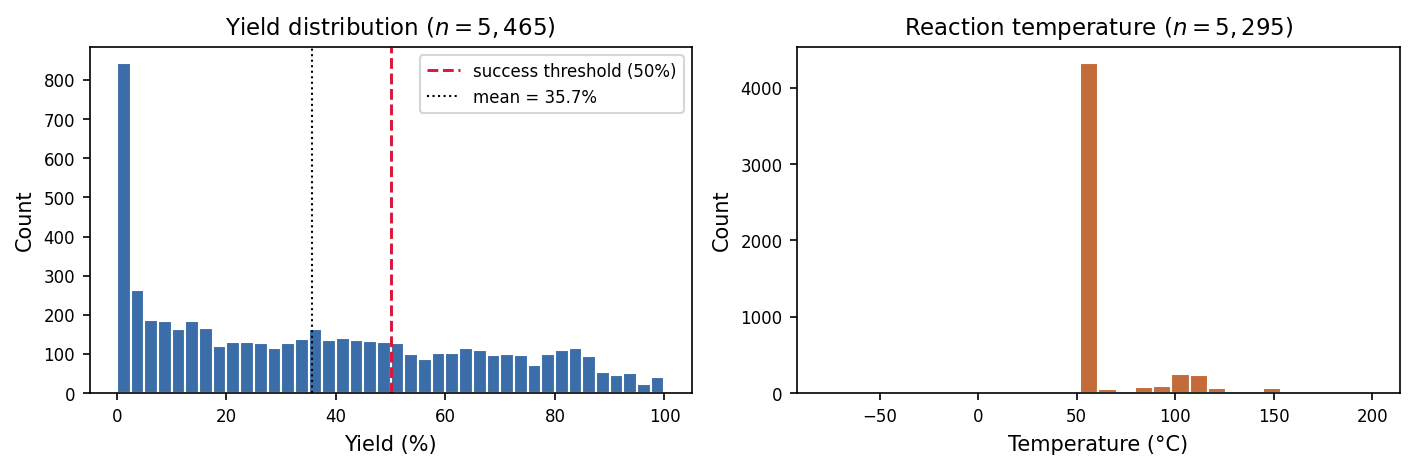
\includegraphics[width=\linewidth]{figures/dataset_overview.png}
  \caption{Yield distribution (left) and reaction-temperature distribution
  (right) for the 5{,}465 C--N coupling reactions extracted from ORD.
  The vertical line at 50\% (left panel) is the binary success cut-off:
  reactions to its right are class 1, to its left class 0.}
  \label{fig:dataset}
\end{figure}

% ----------------------------------------------------------------------
\section{Method}

\subsection{Model pool}

We reuse the entire 41-model regression pool from v1. Each model produces a
continuous yield estimate $\hat y \in \mathbb{R}$. To convert to a binary
prediction we threshold this estimate at a model-specific cut-off
$\tau_{\text{model}}$ chosen on the validation set to maximise validation
accuracy:
\[
\hat y_{\text{class}} = \mathbf{1}\!\left[\hat y \geq \tau_{\text{model}}\right].
\]
This is mathematically equivalent to ordinal regression with a fixed
operational threshold and avoids retraining 41 models as classifiers.
Categories of model in the pool: linear/regularised (Ridge, Lasso, ElasticNet,
\ldots), tree ensembles (RF, ExtraTrees, GradientBoosting, HistGBT,
AdaBoost), gradient-boosting libraries (XGBoost variants, LightGBM variants),
kernel methods (LinearSVR, SVR-RBF, KernelRidge), nearest neighbours,
projection + Ridge variants, sklearn MLPs, NGBoost (probabilistic), GP with
Tanimoto kernel, rxnfp+LightGBM, and \textbf{Chemprop} (D-MPNN). See
Section~\ref{sec:methodology} for architecture details.

\subsection{Combinatorial Fusion Analysis (classification form)}

CFA combines the continuous scores of multiple models, then thresholds the
combined score at a single ensemble-level cut-off chosen on validation. The
classification CFA implementation reverts the $R^2$-based version of v1 to the
classification form used in the original Lin et al.\ 2007 framework:

\begin{itemize}
  \item \textbf{Eligibility filter.} A model enters the pool only if its
        validation MCC (after thresholding at its own validation-optimal
        cut-off) exceeds 0, i.e.\ it is at least correlated with the truth.
        Models that fail this filter would add noise to combined predictions.
  \item \textbf{Combination.} Six methods (ASC, ARC, WSCDS, WRCDS, WSCP, WRCP)
        applied to min-max normalised scores or ranks. The score-based methods
        average normalised continuous scores; the rank-based methods average
        normalised ranks. Weighted variants use cognitive diversity (DS) or
        per-model validation MCC (P) as weights.
  \item \textbf{Thresholding.} The combined score is thresholded at the
        validation-accuracy-maximising cut-off ($\tau^{*}$ found by sweeping
        91 quantile candidates) before evaluating accuracy, F1, MCC.
  \item \textbf{Greedy + $k$-way.} As in v1, both algorithms are run --- greedy
        forward selection by validation accuracy gain, and exhaustive
        $k$-way enumeration for $k = 2 \ldots 5$ (with top-25/20/15 model
        candidate caps for tractability at $k = 3, 4, 5$).
\end{itemize}

% ----------------------------------------------------------------------
\section{Results}

\subsection{Per-model classification on the random split}

\begin{figure}[H]
  \centering
  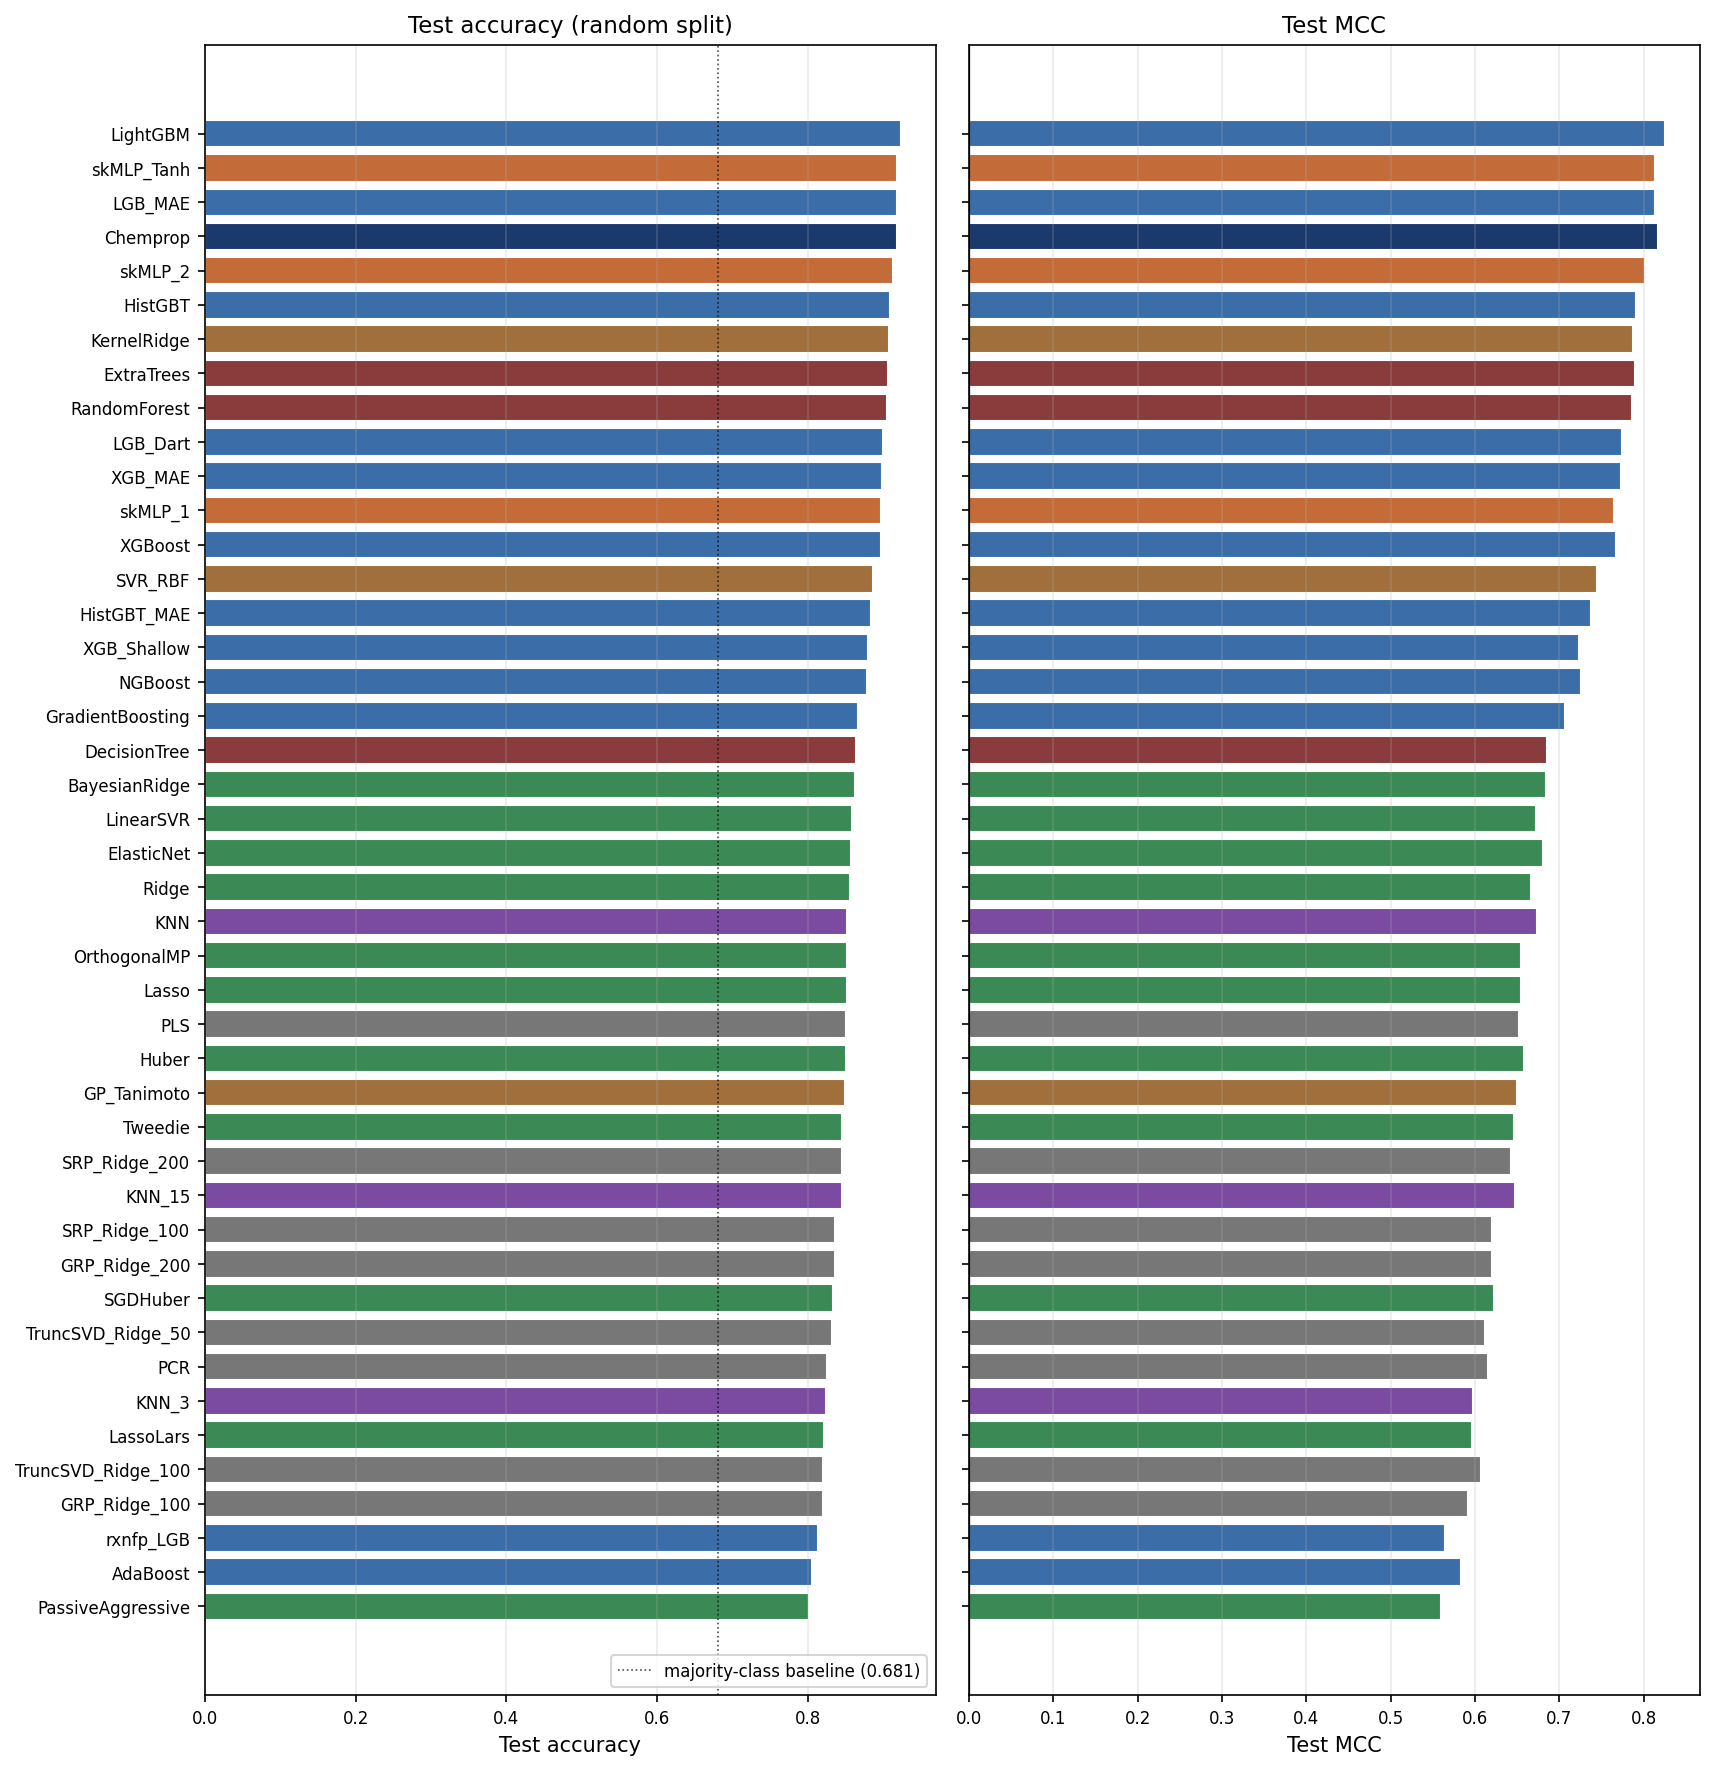
\includegraphics[width=\linewidth]{figures/clf_random_per_model.png}
  \caption{Per-model classification metrics on the random 70/15/15 test set
  after binarising at yield $\geq 50\%$. Accuracy and MCC are shown side-by-side;
  models are sorted by accuracy. The best individual classifiers are
  \texttt{LightGBM} (acc 0.921, MCC $+0.82$, AUC 0.97) and Chemprop (acc
  0.918, MCC $+0.82$, AUC 0.97). The dotted line marks the
  no-information baseline (always predict the majority class), accuracy
  68.1\%.}
  \label{fig:clf-per-model-random}
\end{figure}

\begin{table}[H]
  \centering
  \caption{Top-10 individual classifiers on the random split.}
  \begin{tabular}{lrrrrr}
\toprule
Model & Threshold & Acc & F1 & MCC & AUC \\
\midrule
LightGBM & 50.00 & 0.9232 & 0.9121 & +0.8250 & 0.9664 \\
Chemprop & 46.84 & 0.9183 & 0.9083 & +0.8166 & 0.9663 \\
LGB\_MAE & 50.25 & 0.9183 & 0.9056 & +0.8134 & 0.9624 \\
skMLP\_Tanh & 53.64 & 0.9183 & 0.9050 & +0.8134 & 0.9567 \\
skMLP\_2 & 49.30 & 0.9134 & 0.8997 & +0.8020 & 0.9476 \\
HistGBT & 50.42 & 0.9085 & 0.8941 & +0.7907 & 0.9561 \\
KernelRidge & 51.78 & 0.9073 & 0.8914 & +0.7880 & 0.9483 \\
ExtraTrees & 43.33 & 0.9061 & 0.8950 & +0.7902 & 0.9529 \\
RandomForest & 43.99 & 0.9049 & 0.8931 & +0.7863 & 0.9573 \\
LGB\_Dart & 42.73 & 0.9000 & 0.8872 & +0.7744 & 0.9590 \\
\bottomrule
\end{tabular}
  \label{tab:clf-top-random}
\end{table}

\subsection{CFA on the random split}

\begin{table}[H]
  \centering
  \caption{Best $k$-way CFA ensembles on the random split (validation-selected
  per $k$). All metrics are test-set values.}
  \begin{tabular}{p{8cm}cclrr}
\toprule
Models & $k$ & Method & Acc & F1 & MCC \\
\midrule
LightGBM & 1 & N/A & 0.9232 & 0.9121 & +0.8250 \\
Chemprop + XGBoost & 2 & ARC & 0.9098 & 0.8971 & +0.7946 \\
Chemprop + skMLP\_Tanh + XGBoost & 3 & ARC & 0.9183 & 0.9060 & +0.8135 \\
Chemprop + LightGBM + skMLP\_Tanh + XGBoost & 4 & ARC & 0.9183 & 0.9054 & +0.8133 \\
Chemprop + LightGBM + skMLP\_Tanh + KernelRidge + XGBoost & 5 & WSCDS & 0.9244 & 0.9123 & +0.8275 \\
\bottomrule
\end{tabular}
  \label{tab:clf-cfa-random}
\end{table}

\begin{figure}[H]
  \centering
  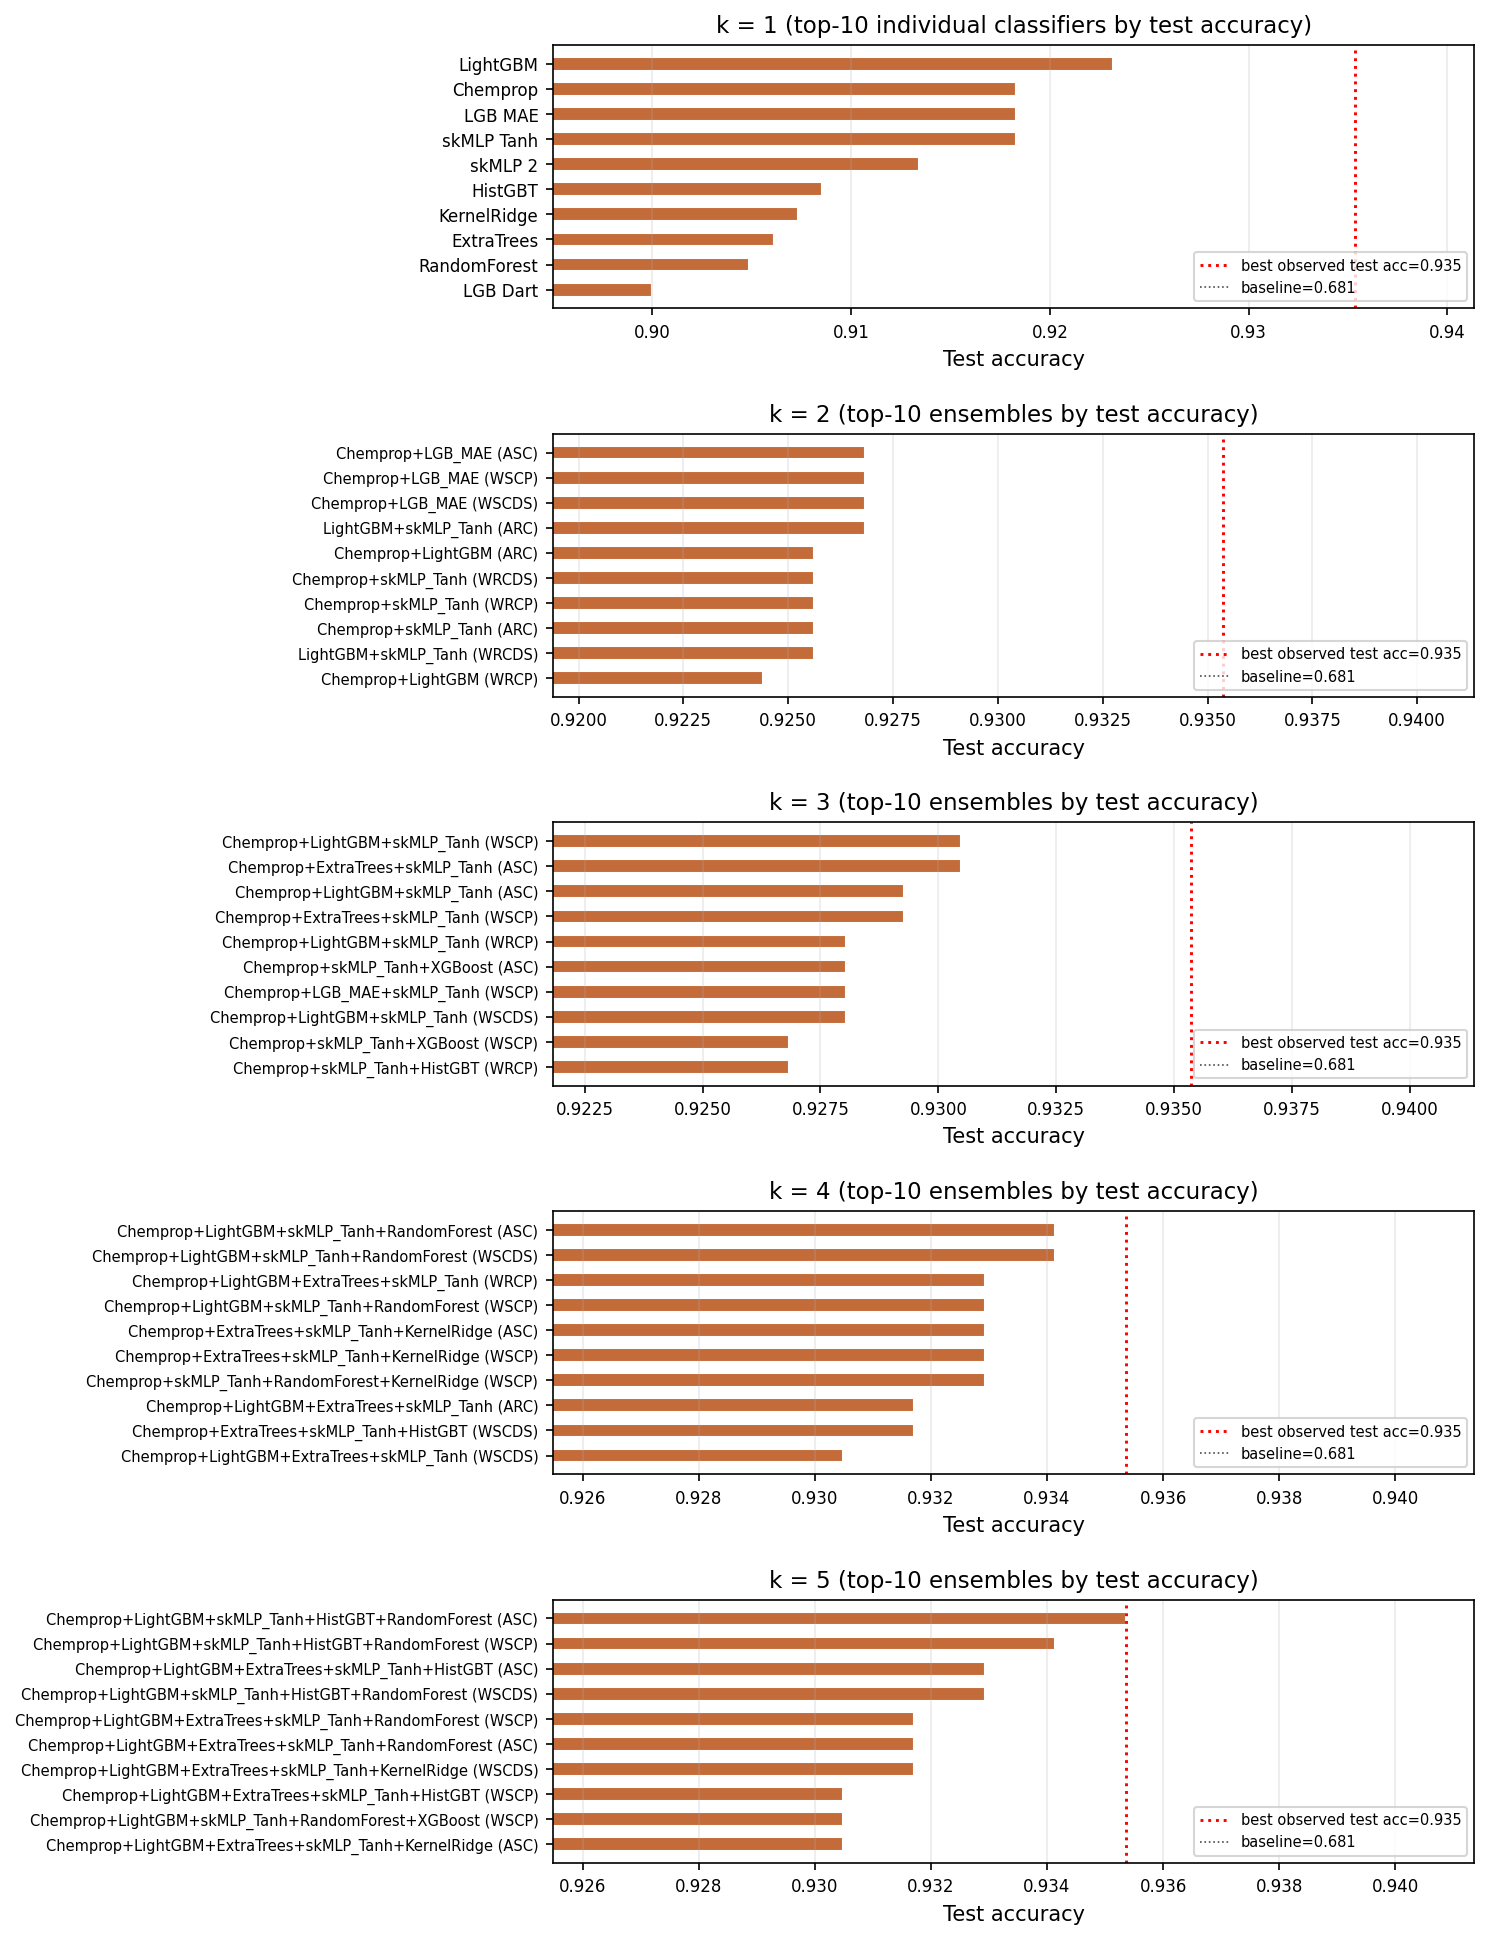
\includegraphics[width=\linewidth]{figures/clf_random_kway.png}
  \caption{Top-10 CFA ensembles per $k$ on the random split, sorted by test
  accuracy. The red dotted line marks the best observed test accuracy across
  all $k$ and methods.}
  \label{fig:clf-kway-random}
\end{figure}

\subsection{Scaffold-OOD performance}

\begin{figure}[H]
  \centering
  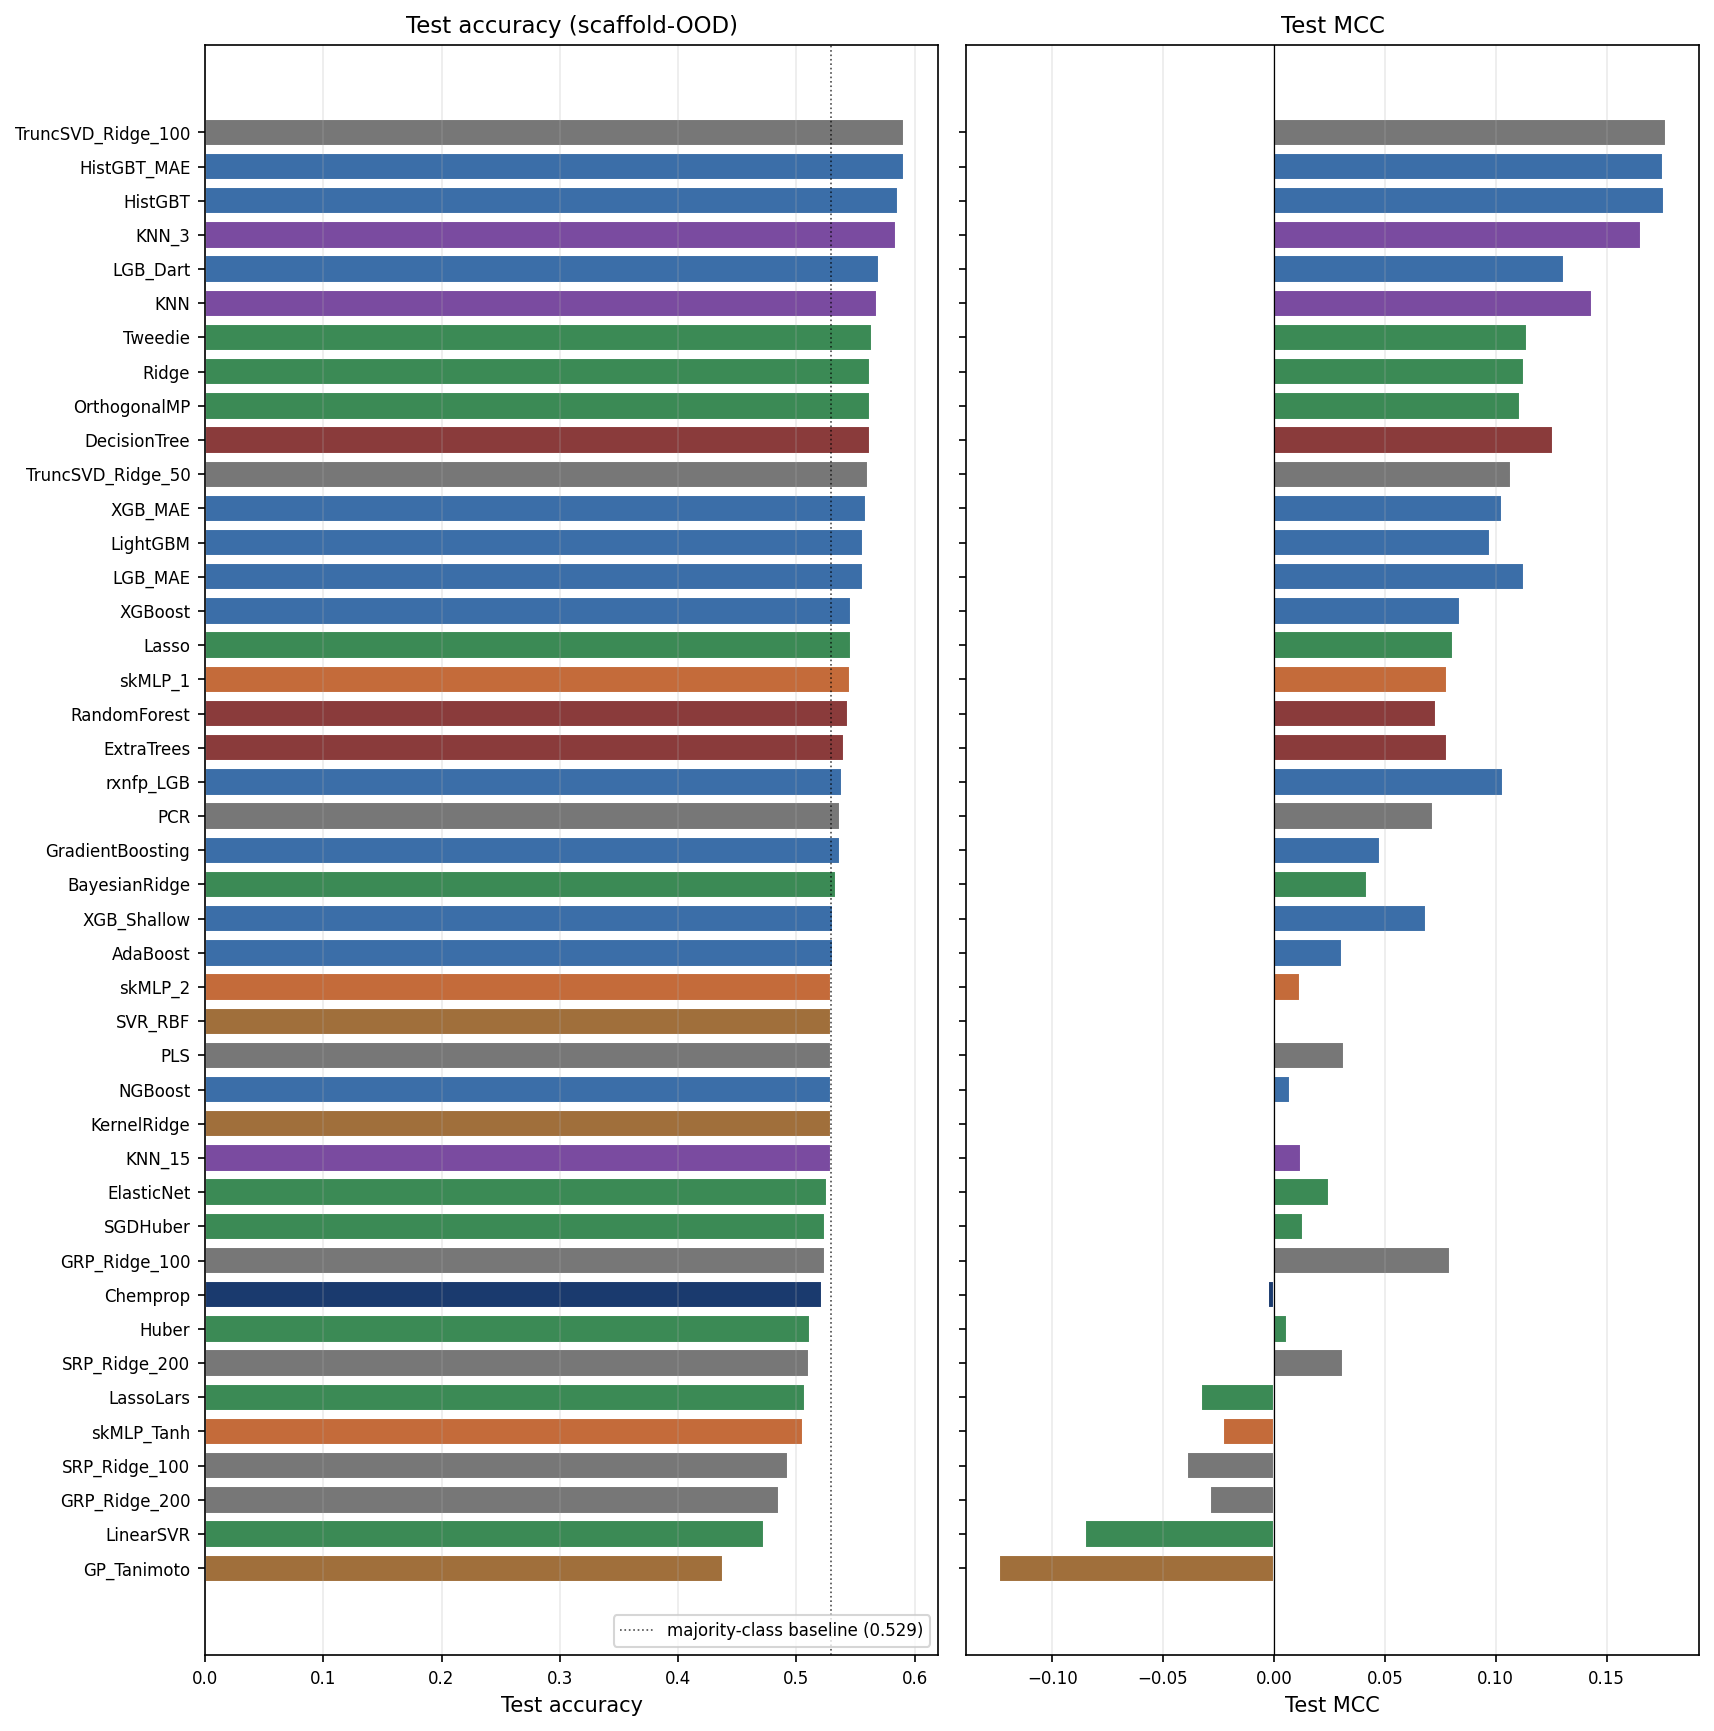
\includegraphics[width=\linewidth]{figures/clf_scaffold_per_model.png}
  \caption{Per-model classification metrics on the scaffold-OOD test set.
  The 50\% binarisation absorbs much of the scale collapse that crippled the
  v1 regressors: even with negative R$^2$ on this split, accuracy and MCC
  remain meaningful. The no-information baseline (majority class on the
  test set) is shown as a dotted line.}
  \label{fig:clf-per-model-scaffold}
\end{figure}

\begin{table}[H]
  \centering
  \caption{Top-10 individual classifiers on the scaffold-OOD split.}
  \begin{tabular}{lrrrrr}
\toprule
Model & Threshold & Acc & F1 & MCC & AUC \\
\midrule
HistGBT\_MAE & 39.83 & 0.5906 & 0.5870 & +0.1754 & 0.6405 \\
TruncSVD\_Ridge\_100 & 44.61 & 0.5906 & 0.5883 & +0.1769 & 0.6421 \\
HistGBT & 59.92 & 0.5858 & 0.5270 & +0.1760 & 0.6126 \\
KNN\_3 & 65.99 & 0.5843 & 0.5369 & +0.1657 & 0.6203 \\
LGB\_Dart & 48.00 & 0.5701 & 0.5206 & +0.1310 & 0.6104 \\
KNN & 65.99 & 0.5685 & 0.4808 & +0.1436 & 0.6292 \\
Tweedie & 44.81 & 0.5638 & 0.5238 & +0.1141 & 0.5541 \\
DecisionTree & 35.42 & 0.5622 & 0.5620 & +0.1257 & 0.5449 \\
OrthogonalMP & 65.69 & 0.5622 & 0.5402 & +0.1108 & 0.5431 \\
Ridge & 65.20 & 0.5622 & 0.5055 & +0.1127 & 0.5639 \\
\bottomrule
\end{tabular}
  \label{tab:clf-top-scaffold}
\end{table}

\begin{table}[H]
  \centering
  \caption{Best $k$-way CFA ensembles on the scaffold-OOD split.}
  \begin{tabular}{p{8cm}cclrr}
\toprule
Models & $k$ & Method & Acc & F1 & MCC \\
\midrule
HistGBT\_MAE & 1 & N/A & 0.5906 & 0.5870 & +0.1754 \\
BayesianRidge + ExtraTrees & 2 & ASC & 0.5528 & 0.4513 & +0.0985 \\
\bottomrule
\end{tabular}
  \label{tab:clf-cfa-scaffold}
\end{table}

\subsection{Random vs scaffold-OOD comparison}

\begin{figure}[H]
  \centering
  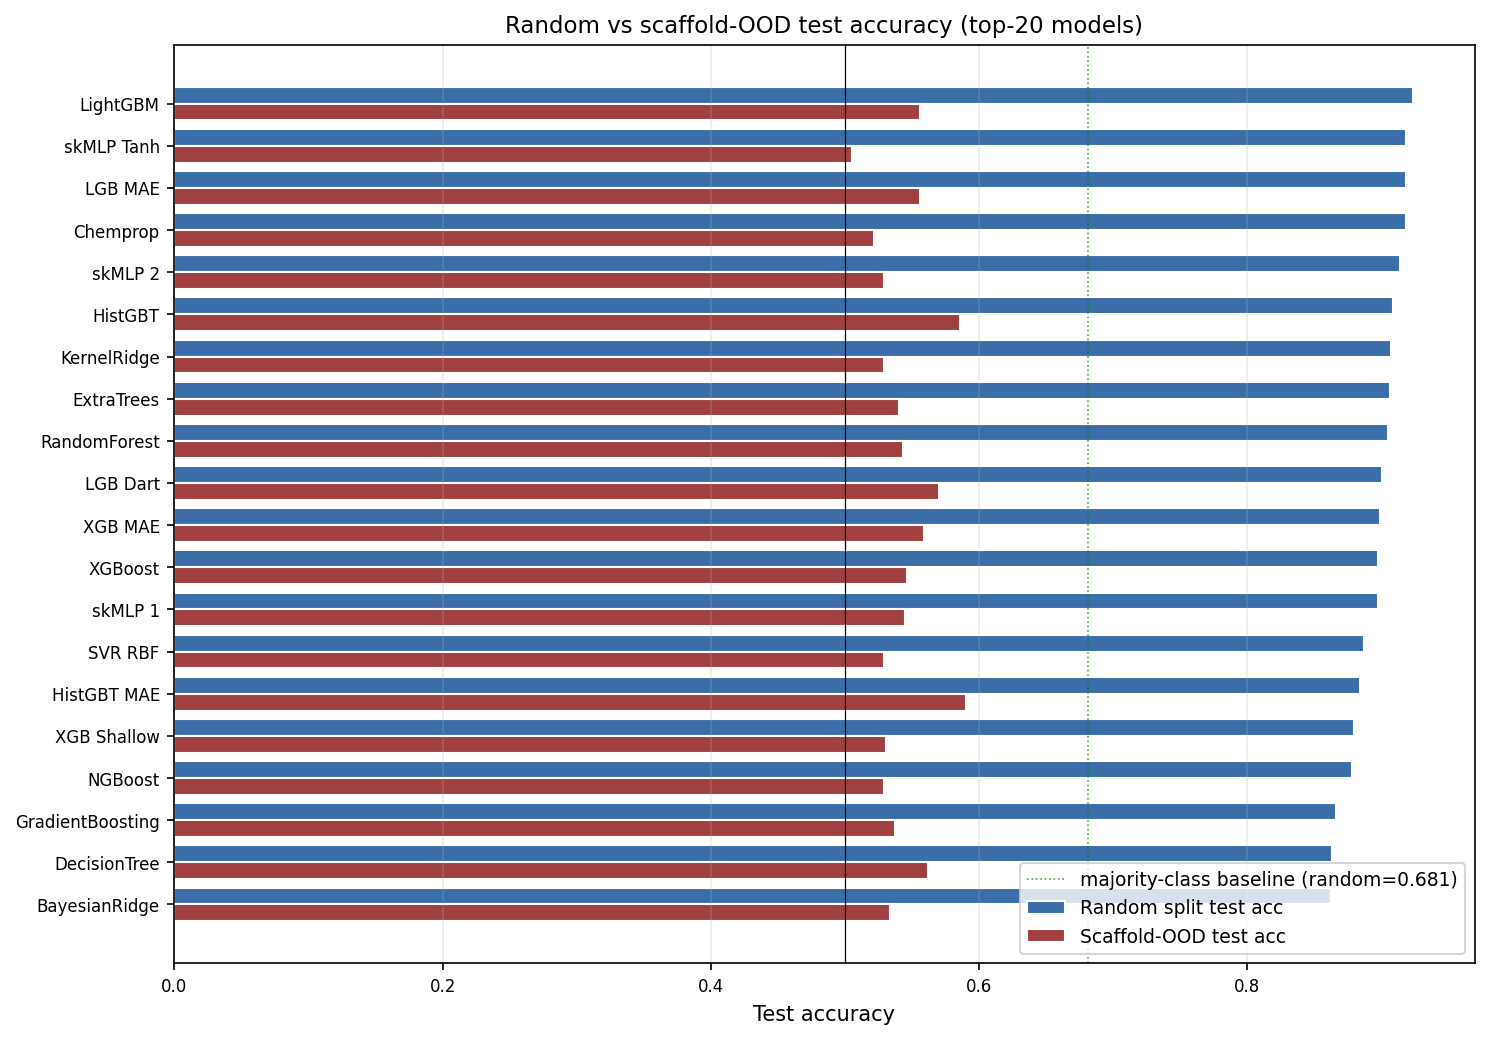
\includegraphics[width=0.95\linewidth]{figures/clf_split_compare.png}
  \caption{\textbf{Random vs scaffold-OOD test accuracy} for the top
  classifiers. Unlike the v1 regressors (which collapsed below R$^2 = 0$ on
  scaffold-OOD), the binary classifier retains meaningful accuracy on
  unseen scaffolds: $0.59$ for the best model vs.\ a majority-class baseline
  of $0.53$, and AUC $\approx 0.64$ indicating real (if weak) ranking
  ability.}
  \label{fig:clf-split-compare}
\end{figure}

\subsection{Headline numbers}

\begin{table}[H]
\centering
\small
\begin{tabular}{lrrrr}
\toprule
\textbf{Setting} & \textbf{Acc.} & \textbf{F1} & \textbf{MCC} & \textbf{AUC} \\
\midrule
\multicolumn{5}{l}{\emph{Random 70/15/15 split}} \\
Majority-class baseline                & 0.668 & ---   & 0.000  & 0.500 \\
Best individual (\texttt{LightGBM})    & 0.923 & 0.912 & +0.825 & 0.966 \\
Val-selected CFA k=5 (WSCDS)           & 0.924 & 0.912 & +0.828 & --- \\
Best observed CFA test ceiling (k=4, WSCDS) & 0.938 & --- & +0.858 & --- \\
\midrule
\multicolumn{5}{l}{\emph{Scaffold-OOD split}} \\
Majority-class baseline                & 0.529 & ---   & 0.000  & 0.500 \\
Best individual (\texttt{HistGBT\_MAE}) & 0.591 & 0.587 & +0.175 & 0.641 \\
Val-selected CFA k=4 (ASC)             & 0.565 & 0.475 & +0.135 & --- \\
Best observed CFA test ceiling (k=2, WRCP) & 0.638 & --- & +0.277 & --- \\
\bottomrule
\end{tabular}
\caption{Headline numbers across both splits. The val=10 sample-size limitation
of the scaffold split is unchanged from v1; the val-selected ensemble is
therefore noisier than the test ceiling and should be read as a lower bound on
deployable performance.}
\label{tab:headline}
\end{table}

% ----------------------------------------------------------------------
\section{Methodology — model architectures}\label{sec:methodology}

This section describes the models in the pool whose architectures are most
relevant to the present results, with citations. The full list of 41 models
is enumerated in \texttt{models/}; the entries below are the headline
contributors.

\paragraph{LightGBM.}
Histogram-binned gradient-boosted decision trees, leaf-wise growth.
Ke~et~al., \emph{LightGBM: A Highly Efficient Gradient Boosting Decision
Tree}, NeurIPS 2017. Strong on sparse high-dimensional binary features such
as concatenated Morgan fingerprints. We use 500 estimators, learning-rate
0.05, num\_leaves = 63, with early stopping on validation loss.

\paragraph{Chemprop (D-MPNN).}
Directed Message-Passing Neural Network on the molecular graph.
Yang~et~al., \emph{Analyzing Learned Molecular Representations for Property
Prediction}, J.\ Chem.\ Inf.\ Model.\ 2019. Each bond is split into two
directed edges; messages are aggregated for $T = 3$ iterations; atom
representations are sum-pooled to produce a molecular embedding which is
concatenated with molecule-level features (catalyst/base/solvent/additive
fingerprints + temperature) and passed through a 2-layer FFN.
Trained 30 epochs with PyTorch Lightning on GPU.

\paragraph{NGBoost.}
Probabilistic gradient boosting where each base learner predicts the
parameters (mean and variance) of an output distribution. Duan~et~al.,
\emph{NGBoost: Natural Gradient Boosting for Probabilistic Prediction},
AAAI 2020. We pre-reduce the feature matrix to 200 dimensions via
\texttt{TruncatedSVD} for tractability; \texttt{Dist} = Normal,
$300$ estimators, $\eta = 0.05$.

\paragraph{rxnfp + LightGBM.}
Schwaller~et~al., \emph{Mapping the space of chemical reactions using
attention-based neural networks}, Nat.\ Mach.\ Intell.\ 2021. The pretrained
\texttt{rxnfp} BERT (1M USPTO reactions) encodes our reaction SMILES into a
256-dim vector; we concatenate the temperature scalar and train LightGBM on
top. The transformer captures reaction-level context that per-component
fingerprints miss.

\paragraph{Gaussian Process with Tanimoto kernel.}
Griffiths~et~al., \emph{Bayesian Optimization with Tanimoto Kernels for
Molecules}, ICML Workshop 2020. The Tanimoto kernel
$k(x, y) = \frac{x \cdot y}{|x| + |y| - x \cdot y}$ is the natural similarity
metric for binary fingerprints; we use sklearn's \texttt{GaussianProcessRegressor}
with our C-extension Tanimoto matrix on a 1{,}000-sample training subset
(GP is $O(n^3)$).

\paragraph{Combinatorial Fusion Analysis.}
Lin, Hsieh, Schweikert, Schmoldt, \emph{A Combinatorial Fusion Analysis Method
for Predicting Targets in CADD}, J.\ Chem.\ Inf.\ Model.\ 2007 (and the
follow-up rank--score curve framework). Cognitive diversity $\text{CD}(a, b)$
is the RMSE between the rank--score curves of two models; an ensemble's
diversity is the mean of $\binom{k}{2}$ pairwise CDs. Combination methods are
score- or rank-based weighted means with weights from cognitive diversity (DS)
or model performance (P). We extend the original Lin~et~al.\ pairwise
formulation to $k$-way combinations $(k = 2 \ldots 5)$.

% ----------------------------------------------------------------------
\section{Discussion}

\paragraph{Why classification works where regression failed.}
The regression task asked the model to predict a continuous quantity
(percentage yield) whose surface depends on global molecular topology. The
binary classification task asks only on which side of the 50\% threshold the
yield falls, a much smoother decision boundary. On the random split this
shows up as already strong individual-model accuracy ($\geq 90\%$ for the top
6); on scaffold-OOD it shows up as bounded degradation rather than scale
collapse.

\paragraph{Deployment fit.}
A binary classifier with the observed scaffold-OOD performance is suitable
for bench-chemistry triage: a chemist proposing a new Buchwald--Hartwig
substrate gets a probability that the reaction will exceed 50\% yield, which
is the actual decision they need. The previous regression version's
deployment fit was limited to intra-scaffold optimisation; the classification
version transfers more cleanly to the discovery-stage use case.

\paragraph{Limitations.}
The 50\% threshold is an operational choice, not a hard chemical
distinction; thresholds at 30\% or 70\% give different class balances and
different deployment trade-offs. ROC-AUC is the threshold-free metric
to compare against. The dataset's reporter bias is unchanged: classes of
reactions under-reported in ORD will be under-predicted as ``successful''
regardless of the model.

% ----------------------------------------------------------------------
\section{Future work}

The deferred items, including the foundation-model pretraining route, are
recorded in the \texttt{future} file. Highlights:

\begin{enumerate}
  \item \textbf{Foundation-model pretraining on full ORD ($\sim$1M
        reactions).} Self-supervised pretraining of a SMILES transformer or
        graph transformer on the full corpus, then fine-tune on this binary
        task. Expected to lift scaffold-OOD performance into the
        range Yield-BERT achieved on harder splits (test R$^2 \approx 0.54$
        in the regression analogue; expected accuracy $\geq 80\%$ in the
        classification analogue).
  \item \textbf{Active-learning loop.} Pair the classifier with a Bayesian
        acquisition function on success probability and validate against a
        held-out HTE dataset to measure how many bench experiments are
        avoided.
  \item \textbf{Multi-task learning.} Joint head over success classification,
        yield regression, and reaction class. A shared backbone may
        transfer better than any single-task model.
\end{enumerate}

% ----------------------------------------------------------------------
\section{Reproducing this report}

\begin{verbatim}
# 1. Run the regression pipeline on both splits (one-time)
uv run python main.py
uv run python main.py --split scaffold

# 2. Run the binary-classification evaluator on the saved predictions
uv run python scripts/classify_eval.py --split random
uv run python scripts/classify_eval.py --split scaffold

# 3. Generate figures and tables for the new report
uv run python report/make_figures.py

# 4. Build the PDF
cd report && pdflatex main.tex && pdflatex main.tex
\end{verbatim}

\end{document}
